
\section{Background and Motivation}
In this section, we illustrate the benefits of cross-platform computing and introduce state-of-the-art frameworks that are designed to support it. Then we discuss our motivation for developing CLIC on the cloud and lists the challenges.

\subsection{The Demand for Cross-Platform Workflows}

Modern data analysis generally adopts a workflow that includes tasks from multiple domains, such as data cleaning, relational data analysis, and machine learning. The involved tasks in such a workflow are beyond the capability of one single platform~\cite{tsoumakos2013case, gadepally2015d4m}. Data processing platforms are generally developed for certain workloads, and applications often need to utilize multiple platforms to fulfill their computing requirements ~\cite{wang2017myria, lu2019multi, tan2017enabling}. Moreover, with different formats of incoming data, e.g., streaming data, graph data, there are also targeted platforms such as Flink and Giraph.

Taking real-time recommendation as an example (Figure~\ref{fig:recommend-workflow}), its workflow consists of an offline phase and an online phase. The offline phase preprocesses historical transaction records and extracts features, which requires massive distributed data processing, and then the features are used to train a deep learning recommendation model. The online phase collects and analyzes time-series streaming data and uses incremental learning to calibrate the model. The recommendation model is used to make product recommendations based on user browsing behaviors~\cite{huang2015tencentrec}. A common architecture of this workflow is shown in Figure \ref{fig:recommend-workflow} in which the offline records processing phase is taken by a distributed processing framework like Spark while the model is trained using Tensorflow. The online phase may adopt Flink for online stream processing and then uses Tensorflow for incremental learning. This case demonstrates the necessity of adopting multiple platforms in building an application workflow.


Besides the demand for capabilities for the involved task processing, leveraging different platforms can also speed up the performance of a workflow. By decomposing a workflow as multiple tasks and deploying them on platforms optimized for the particular workloads, the overall performance can be improved~\cite{agrawal2016rheem, gog2015musketeer, gittens2018accelerating, tan2017enabling, anderson2017bridging}. For example, the performance of Word2Vec~\cite{mikolov2013efficient} algorithm on different platforms is shown in Figure \ref{fig:base-w2v}, where SparkML is faster than single-machine frameworks PyTorch and gensim when the corpus is large but gets slower when the corpus becomes small. The performance advantage stems from Spark’s bulk synchronous model, where a dataset is split and stored on multiple nodes to increase parallelism~\cite{zaharia2016apache}. It benefits distributed algorithms with little communication overheads, such as Word2Vec~\cite{stergiou2017distributed}. 
Another instance is shown in Figure \ref{fig:base-pca} where the execution time of Spark is always exponentially higher than other platforms for principal component analysis (PCA).  The PCA algorithm is an iterative algorithm that contains frequent multiplication on block matrices in extracting eigenvector~\cite{gittens2016matrix}. Its low performance on Spark is attributed to the distributed coordination overheads, including scheduler delays, stage initialization costs, and task start delays~\cite{gittens2018accelerating, bosagh2016matrix}.
%Another case is that an algorithm can be decomposed into multiple parts, each of which is deployed to a more economical platform to enhance the overall performance. For instance, Rheem~\cite{agrawal2016rheem} abstracts Stochastic Gradient Descent (SGD) algorithm to an iteration and a processing phase. It then deploys iterations at JavaStream to avoid frequent synchronization overheads in Spark and deploys the other phase at Spark, which finally acquires a significant performance improvement.


\begin{figure}
  \centering
  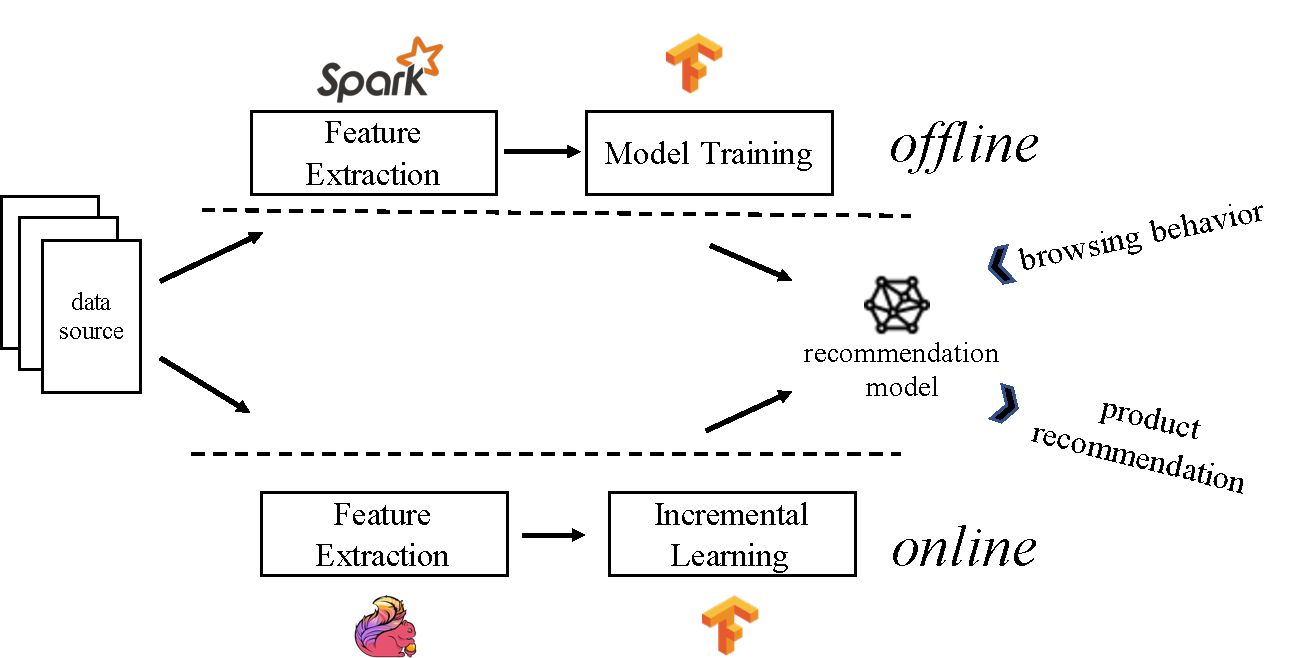
\includegraphics[width=0.8\linewidth]{figures/recommendation.pdf}
  \caption{Workflow of real-time recommendation}
  \label{fig:recommend-workflow}
\end{figure}

\begin{figure}
  \centering
  \subfigure[Word2Vec]{
  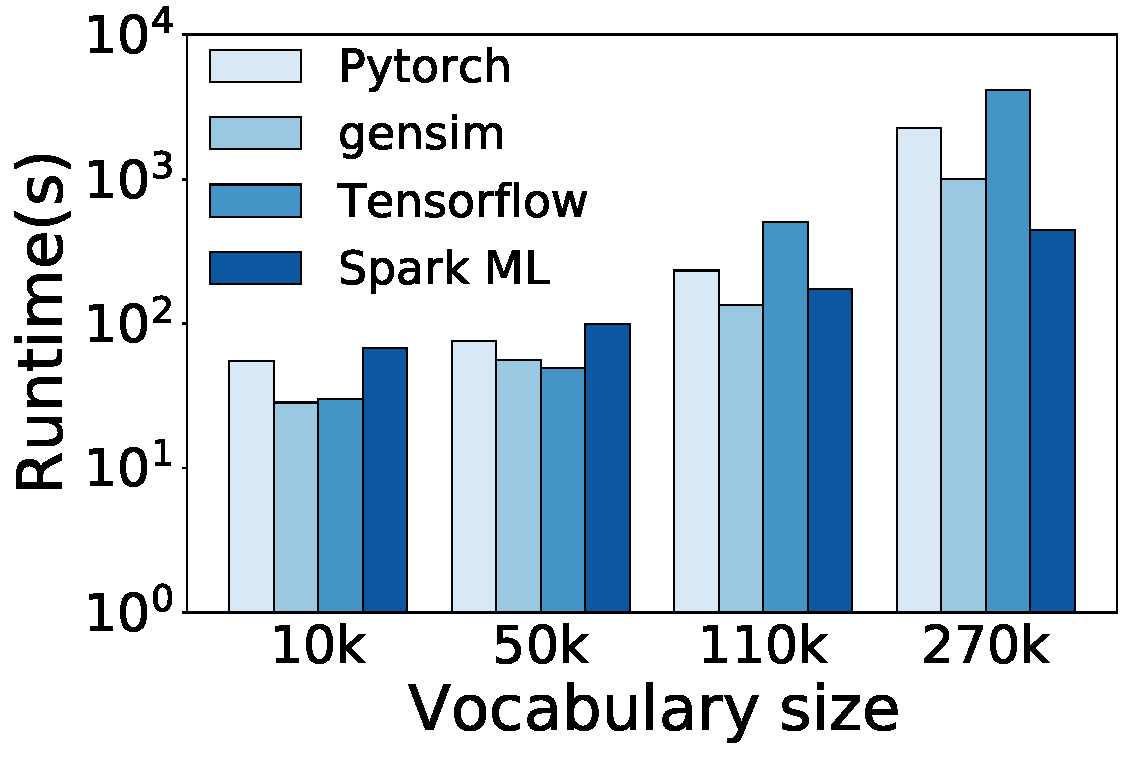
\includegraphics[width=0.45 \linewidth]{figures/chp2-word2vec.pdf}
  \label{fig:base-w2v}
  }
  \subfigure[PCA]{
  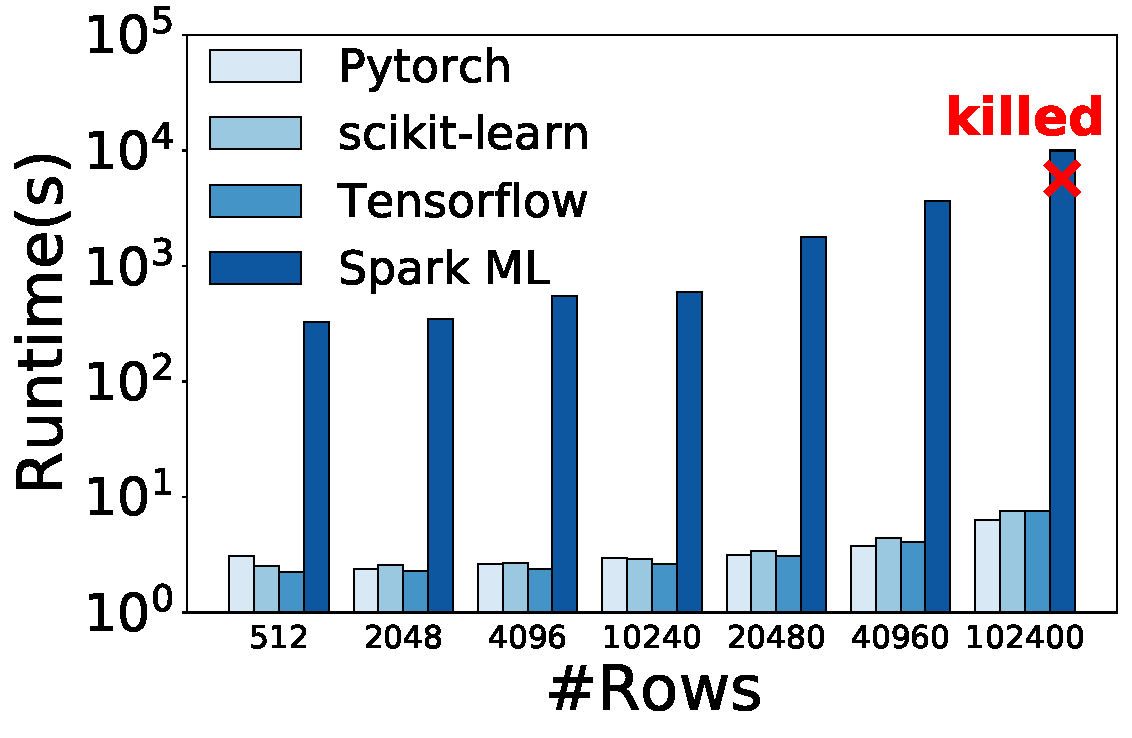
\includegraphics[width=0.45 \linewidth]{figures/chp2-PCA.pdf}
  \label{fig:base-pca}
  }
  
  \caption{Performance impact from different platforms}
  \label{fig:hetero}
%  \vspace{-20pt}
\end{figure}




\subsection{State-of-the-art Cross-Platform Frameworks}

Cross-platform computing can bring notable benefits, while building such a workflow faces several difficulties. Firstly, developers are required to learn the usages and programming models of the involved platforms, resulting in a high learning curve~\cite{gadepally2016bigdawg}. Secondly, to achieve the desired performance, developers need to choose appropriate platforms according to the workflow~\cite{agrawal2016rheem,hutchison2017laradb,gog2015musketeer}.
This gives rise to the study of the support for cross-platform computing, where a number of cross-platform frameworks are developed~\cite{tsoumakos2013case, tan2017enabling, lu2019multi,gittens2018accelerating}.
These works aim at addressing different issues, and we classify the state-of-the-art approaches into two categories.

\textbf{A unified execution engine} A class of work, e.g., BigDL~\cite{dai2019bigdl}, Spark~\cite{zaharia2016apache}, Ray~\cite{moritz2018ray} and LaraDB~\cite{kunft2019intermediate}, develops a big ecosystem and an universe API for performing tasks of a variety of domains. For instance, Spark’s execution engine supports not only map-reduce-style computing but also graph computing, machine learning, and SQL queries. This approach reduces programming efforts and mitigates the communication and data transfer overhead between tasks that were supposed to be deployed on two different platforms. However, it suffers from side effects of "one size fits all”. For example, Spark achieves suboptimal performance for specific tasks due to the different requirements for underlying storage and computing engines~\cite{anderson2017bridging, gittens2016matrix, gittens2018accelerating, dai2019bigdl}, such as the PCA algorithm shown in Figure \ref{fig:base-pca}. %Another issue is that it is hard to utilize existing platforms due to different programming languages or underlying architectures, demanding nontrivial development efforts.

\textbf{A framework that integrates existing platforms}    Another approach is to build a cross-platform framework that federates existing data processing platforms and provides a common interface to facilitate building cross-platform workflows~\cite{gog2015musketeer, agrawal2016rheem, hausenblas2013apache, beam2017apache, wang2017myria, dziedzic2016data}. Representative works include Rheem~\cite{agrawal2016rheem} and Musketeer~\cite{gog2015musketeer}. 
These frameworks provide an abstraction for building workflows. For cross-platform computing, a cost model is typically used to estimate the running time of each operator and select platforms that can improve the performance of a workflow. 
Specifically, Rheem uses a Java-based driver to drive workflow execution where tasks can only be executed on platforms with Java interface. This design excludes lots of well-known platforms such as PyTorch and Tensorflow. Differently, Musketeer translates front-end descriptions to common intermediate representations and then generates codes for selected platforms. In the paper, only SQL-like queries and vertex-centric graph are its supported front-ends, requiring significant development efforts to support complex data science workflows.

Previous works have enhanced cross-platform computing in multiple aspects and helped build efficient data science applications. Between the two types of approaches, the cross-platform framework is able to utilize existing data processing platforms which feature mature communities and well-tuned performance. Therefore, we believe it is a promising direction for applying cross-platform computing to data science.


\subsection{Deploying Data Analysis Workflows on the Cloud}

With the fast development of cloud computing, data science applications have been migrating to cloud for higher availability, higher scalability, and lower cost.
Cloud infrastructure provides virtualization technologies that encapsulate programs, dependencies and system settings in containers, where an instance can run with flexible resources and independent environments~\cite{wang2017myria}. Moreover, platforms contain different dependencies. To allow flexible task deployment, each node in a cluster should be installed with dependencies of all platforms, which incurs nontrivial maintenance overhead. 
To address these issues, cloud is a good candidate to meet the requirements in building cross-platform data analysis workflows.
To enable data analysis on the cloud, there are several requirements and challenges to address for a competent system.

\textbf{Agile platform integration} For the data analysis workloads that exhibits huge variance, there are a large amount of data processing platforms designed for specific workloads. Moreover, new data processing platforms are constantly emerging. To meeting users' demands and benefits the performance advantage from the new platforms, cross-platform frameworks need to adapt to the changes, which makes agile platform integration an essential feature. However, previous frameworks are designed with a tightly coupled architecture in which tasks of a workflow are executed by one driver program~\cite{balalaie2015migrating}. Consequently, integrating a new platform is expensive, which needs to rebuild, test, and deploy the entire project every time.

%????? \textbf{Platform management} Most data processing platforms are open source projects under fast development. Platforms frequently add new programming interfaces and features and remove old ones, which makes developed functions and programs can only be executed in specific versions. Therefore, cross-platform frameworks should be able to deploy a developed operator on the corresponding version of its dependent platform.

\textbf{Robust platform selection} System software and hardware configurations have a huge impact on the performance of data processing~\cite{mattson2019mlperf}. Cloud providers generally offer different cloud instances with flexible hardware resources like the number of virtual CPU, memory capacity and network speed. Therefore, workflows from different users run in a variety of virtual hardware configurations and cluster scale, which influences platform selections for workflow operators~\cite{}. Although previous approaches adopt models in platform selection, their models are trained under specific hardware and software settings and cluster scale. Consequently, it is hard to adopt such approaches in the cloud environment which can easily fail with a changing environment. Overall, all the factors lead to the requirement for an efficient and robust platform selection algorithm for the cloud.


\textbf{Flexible Scaling} With tasks like data cleaning, filtering, and feature extraction, the input data for tasks in a workflow can be of huge variance. Therefore, a workflow demands different amounts of computational resources in its lifetime, which needs to be dynamically allocated at runtime. Moreover, flexibly scheduling tasks on specific nodes can help enhance the hardware utilization [osdi20xiao]. The architecture of current cross-platform frameworks tightly couple the development and deployment of platforms with the framework itself, and they typically initialize resources, like nodes in a cluster, before the workflow execution and occupy the resources throughout a workflow's life time. As a result, tasks of a workflow have to be executed as one instance, which leads to the same execution environment and hardware resources for all tasks. This design cannot adapt to changing workloads, resulting in either resource overprovisoning or low performance.

Considering all the potential issues in running cross-platform workflows on the cloud, it calls for a redesign of the architecture to adapt to the cloud environment for higher resource utilization.
